\subsection{Hardware Constraint}
\begin{itemize}
	\item iOS or Android smartphones
	\item PC/Mac support
	\item WiFi and web connection
	\item GPS
\end{itemize}

\subsection{Functional Requirements}



\begin{itemize}
	\item[G1] Allow the user to add an appointment
	\subitem[G1.1] The user can add the date of the appointment through a calendar
	\subsubitem[R1.1.1]The application must provide the user with a calendar in order to choose the date
	\subitem[G1.2] The user can select the location through a map
	\subsubitem[R1.2.1]The application must provide a map in order to obtain the GPS coordinates
	\subitem[G1.3] The appointment must be processed by the system
	\subsubitem[R1.3.1]The application accepts only appointments with at least date, starting time, ending time, location and description with no overlapping with other appointments
	\subsubitem[R1.3.2]The appointment is processed and registered if it doesn’t overlap with other appointments of the logged user
	\subsubitem[R1.3.3]The location is solved completing it with GPS coordinates and address using external map services
	\subsubitem[R1.3.4]The application must notify the user about possible errors that prevents the processing of the appointment to the user
	\item[G2] - Provide a route to the user for reaching the appointments
	\subitem[G2.1] The user must reach on time his/her appointments
	\subsubitem[R2.1.1]The arrival time must precede the starting time of the appointment
	\subsubitem[R2.1.2]The starting time of the route must be after the ending time of the previous appointment
	\subsubitem[R2.1.3]The application must send a notification to the user to remind him about the next travel
	\subitem[G2.2] The user can choose the starting location and time of the route
	\subsubitem[R2.2.1]From the location and the ending time of the previous appointment (if it exists)
	\subsubitem[R2.2.2]From a personalized location and time
	\subsubitem[R2.2.3]From the current location and time
	\subitem[G2.3] Generate routes according to the preferences of the user
	\subsubitem[R2.3.1]All global preferences of the user must be satisfied
	\subsubitem[R2.3.2]The user can add one preference profile for the current appointment
	\subsubitem[R2.3.3]The preferences provided in the preference profiles are constraints connected by logical AND
	\subitem[G2.4] The application provides a route for each objective, minimizing each of these attributes: length, duration, number of changes, carbon footprint
	\subsubitem[R2.4.1]Each route provided must indicate starting and ending time, IDs of public transportation to use, distance, carbon footprint, paths
	\subsubitem[R2.4.2]The application must remind the user about the start of the route
	\subsubitem[R2.4.3]The user can order the result according to
	\begin{enumerate}

		\item Length
		\item Duration
		\item Number of changes
		\item Carbon footprint
		\item The public transport timetables are obtained by contacting external services
	\end{enumerate}
	\subsubitem[R2.4.4]The available means of transport are
	\begin{enumerate}

		\item Private car
		\item Bicycle
		\item On foot
		\item Public transportation
		\item Bus
		\item Tram
		\item Underground
		\item Train
		\item Taxi
		\item Car sharing
		\item Bike sharing
	\end{enumerate}
	
	\subitem[G2.5] Always provide a route
	\subsubitem[R2.5.1]If there are no routes that satisfy all the requirements, search again allowing an arrival time after the starting time of the appointment
	\subsubitem[R2.5.2]Report the arrival delay with a warning
	\subitem[G2.6] During strike days, public transportation must not be available
	\subsubitem[R2.6.1]If a society emerges to be striking, its services must not be available for the calculation of the route
	\subitem[G2.7] Report unfavorable weather conditions
	\subsubitem[R2.7.1]Add a weather warning to the route if part of it is on foot or bicycle in locations or hours in which unfavorable weather conditions are expected during the calculation of the route
	\subsubitem[R2.7.2]Unfavorable weather conditions are rainfalls or temperature under 3 C
	\subsubitem[R2.7.3]Weather forecasts are requested through external services
	\subitem[G2.8] Update unfavorable weather conditions
	\subsubitem[R2.8.1]The user must be logged
	\subsubitem[R2.8.2]Update the weather conditions of the saved routes every 6 hours and notify unfavorable weather conditions on routes with parts on foot or bicycle if not already done previously
	\subitem[G2.9] The user can save one route among the shown ones
	\subsubitem[R2.9.1]The user can choose anyone of the provided routes
	\subsubitem[R2.9.2]The choice must be saved in the database if the user is logged
	\item[G3] Allow the user to sign up into the application
	\subitem[G3.1] The registration must allow the univocal recognition of the user
	\subsubitem[R3.1.1]The registration is valid if it contains at least First Name, Family Name, date of birth, fiscal code, telephone number, e-mail address, valid password
	\subsubitem[R3.1.2]The fiscal code is valid if it agrees with name, family name and date of birth
	\subsubitem[R3.1.3]The e-mail address is valid if it is not already taken in the database
	\subsubitem[R3.1.4]The password is valid if it contains at least 6 letters
	\subsubitem[R3.1.5]The system can accept only valid registrations
	\item[G4] Allow the user to log in
	\subitem[G4.1] The system allow the login through e-mail and password
	\subsubitem[R4.1.1]The user can request for the access into the application using e-mail and password
	\subsubitem[R4.1.2]The access is guaranteed only if e-mail and password prove to be linked to an account
	\subsubitem[R4.1.3]The application must notify the user about the outcome of the login
	\subitem[G4.2] The application allow the login through telephone number
	\subsubitem[R4.2.1]The user can request for the access using the telephone number
	\subsubitem[R4.2.2]The system must be able to send an SMS to the provided number with a verification code of 4 digits
	\subsubitem[R4.2.3]The user can complete the login if the verification code inserted by the user matches the one generated by the system
	\item[G5] Allow the user to add his own preferences
	\subitem[G5.1] The user must be logged
	\subitem[G5.2] The preferences are synchronized between the application and the database
	\subsubitem[R5.2.1]Each modification to the user settings must be reflected in the update of the database
	\subsubitem[R5.2.2]The preferences can be changed only if the user is logged
	\subitem[G5.3] The user can chose the available transport means
	\subsubitem[R5.3.1]The subsequent routes can use only the vehicles marked as available in the preferences
	\subitem[G5.4] The user can add a priority to the means of transport
	\subsubitem[R5.4.1]Each mean of transport can have a priority among low, normal and high
	\subsubitem[R5.4.2]While calculating the route, if more vehicles are available for the same path, the one with highest priority is chosen
	\subitem[G5.5] The user can add the maximum length of routes on foot or by bicycle
	\subsubitem[R5.5.1]Distances can be expressed in meters or kilometers
	\subitem[G5.6] For each vehicle the user can choose a time slot of validity
	\subsubitem[R5.6.1]The user can choose one or more time slots of validity for a given vehicle with the possibility of scheduling on a weekly basis and with accuracy of minutes
	\subitem[G5.7] The user can set Flexible Lunch
	\subsubitem[R5.7.1]Given the time slot for the lunch break and its minimum duration, the application must guarantee that, for at least the specified duration, the user is not traveling during that time slot
	\subsubitem[R5.7.2]The minimum duration of a lunch break must not exceed the duration of the chosen time slot
	\subitem[G5.8] The user can add breaks for fixed moments of the day
	\subsubitem[R5.8.1]The insertion of the time slot by the user is mandatory
	\subsubitem[R5.8.2]During the time slot set by a break, no scheduled journey must be in progress
	\subitem[G5.9] The user can add a private car or bicycle
	\subsubitem[R5.9.1]It is needed to indicate the habitual parking zone of the vehicle.
	\subitem[G5.10] The user can organize his preferences in “Preferences Profiles”
	\subsubitem[R5.10.1]The user can include a preference in one or more preferences profiles
	\subsubitem[R5.10.2]If no profile is specified, the preference has global validity
	
	\item[G6] Allow the user to manage his account
	\subitem[G6.1] The user must be able to remove appointments and routes
	\subsubitem[R6.1.1]After removing a appointment, the previous and following routes are removed as well
	\subitem[G6.2] The user must be able to modify appointments and routes
	\subsubitem[R6.2.1]In case of modification of a route, the application will provide the user with a new list of newly generated routes to choose
	\subsubitem[R6.2.2]In case of modification of the starting or ending time or the location of a appointment, the eventually present previous and subsequent routes will be removed
	\subitem[G6.3] The user must be able to delete his account
	\subsubitem[R6.3.1]The removal of the account implies that the system deletes the credentials and all personal data and information of the user
	\item[G7] Allow the user to report events and disservices 
	\subitem[G7.1] The user can report strikes using the application
	\subsubitem[R7.1.1]The user must provide the striking society and report the day of the strike and the starting and ending time
	\subitem[G7.2] The user can report faults, malfunctions and suggestions
	\subsubitem[R7.2.1]The user must indicate the reason of his report with a textual message
	
\end{itemize}



\subsection{Software System Attributes}
\subsubsection{Performance}
The system must answer rapidly to the requests of the users while searching for timetables and calculating the routes. The performance of the system depends also on the response time of the external services.

\subsubsection{Reliability}
The system must be available 24/7. However also in this case the availability of the service depends on the one of external services. The lack of availability of the former can limit the functionalities of the main application
\subsubsection{Security}
Some personal data are stored in the database, so it is necessary to guarantee security over these data.
\subsubsection{Scalability}
The system can be expanded with new external services. It must be designed in such a way that makes possible modifying or adding other services for accessing the timetables, the maps and the weather forecast.
\subsubsection{Accuracy}
The timetables and the estimated length and duration of the routes must be as precise as possible. Also the weather forecast must be updated regularly to provide reliable information.

\subsection{More Non Functional Requirements}

\subsubsection{Licensing}
Front End application will be eventually distributed under Freeware License


\subsection{Scenarios}
	\subsubsection{Scenario 1}
	Bob is looking for a service that allows him to keep track of all his work meetings around Milan. Surfing on web, he finds Travlendar+, so he decides to use that for his schedules. Downloaded the app, from the homepage,  he requests the list of his registered appointments, actually empty. Then, he add a new appointment providing the date and time of beginning and end of meeting, finally, a brief description. He didn’t choose to compile the departure and hour position, so now he can choose five different options to reach the meeting from his actual position. He decide to save the route with lower travel time and waits for the suggested beginning of travel.
	\subsubsection{Scenario 2}
	Alice has a very busy life, but bad memory too, so she has adopted to use Travleandar+ everyday to reminds her all her work and private appointments. Now she decides to make an account to keep synced appointments among all her devices, and have always a backup in case she loses a device. Therefore, she selects the option that permits to create a new account, she fills all fields required to her, including name, surname, FC, email, new username and password. Finally, she logged in from different devices finding her list of appointment up to date.
	\subsubsection{Scenario 3}
	Tracy is a registered user of Travlendar+. She wants to personalize the choice of routes in order to fulfill her needs and preferences. She is already logged in Travlendar+, so she can choose to view and modify her preference profiles through the specific function. She adds a new preference profile providing a name for it, then she creates the flexible launch preference and she sets also a travel pause between 7-8 pm. Finally, she added the new preferences to the just created preference profile. Now she can apply the profile to all new and already setted appointment during their creation or modification.
	\subsubsection{Scenario 4}
	Bob has just been informed about a change in the afternoon meeting. He has already added this meeting appointment in Travlendar+ sometime before. By the appointment view, he chooses the one he wants modified, and he changes only the beginning hour, anticipating that by half an hour, according to new schedule. Now he is asked to choose another among others routes to reach the modified appointment in time.
	
	\subsubsection{Scenario 5}
	Luna is a environmentally conscious person that always tries to help the nature. So she uses Travlendar+ with the objective to minimize her travel carbon footprint. For the last inserted evening appointment, she accidentally selects a route that implies a lot of CO2 emissions, so she wants to change that. She navigates her appointment list, selects the evening appointment and she can select another route among different choices. She finally saves the route that minimize carbon footprint.
	\subsubsection{Scenario 6}
	Alice is afraid of travel alone by train at night because of self security concerns. Therefore she has decided to always avoid trains between 22.00 and 5.00. On Travlendar+, she adds to “default” preference profile a specific rule that permits her to disable a transport means for a specific period of the day. As far the new rule is linked to “default” is always considered in route generation, so she will be never asked to travel by train at night.
	\subsubsection{Scenario 7}
	Tracy has just been notified by Travlendar+ about icy temperatures on the following day. So she decides to change one route of the following day avoiding walking and bicycles. Through the notification, she obtains a list of her routes with walking or bike parts with bad forecast or freezing temperatures, and for each of them, she can choose an alternative path.
	\subsubsection{Scenario 8}
	Bob is the owner of a private car that he would like to use during his travels. Since he is already registered and logged in, he can add, as global preference (to “default” profile) his car, indicating where it is normally parked. By this moment, every new generated route for an appointment can consider the employment of own registered means.
	
	
\subsection{Use case description and diagram}
\begin{figure} [H]
	\centering
	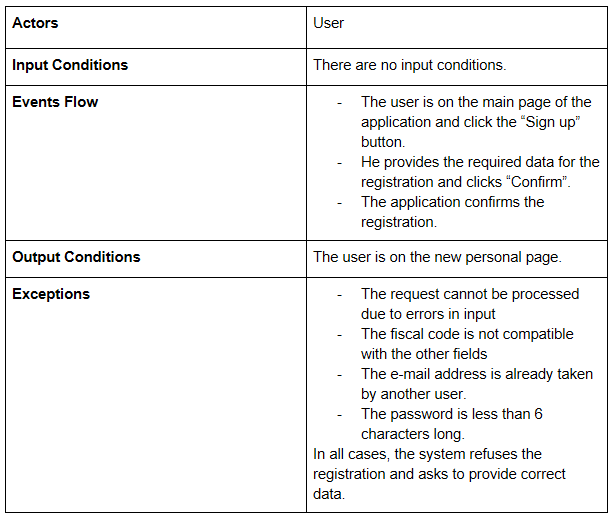
\includegraphics{Images/UseCaseTables/1_user_reg.PNG}
	\caption{\label{fig:useCase1}Use case - User Registration }
\end{figure}

\begin{figure}
	\centering
	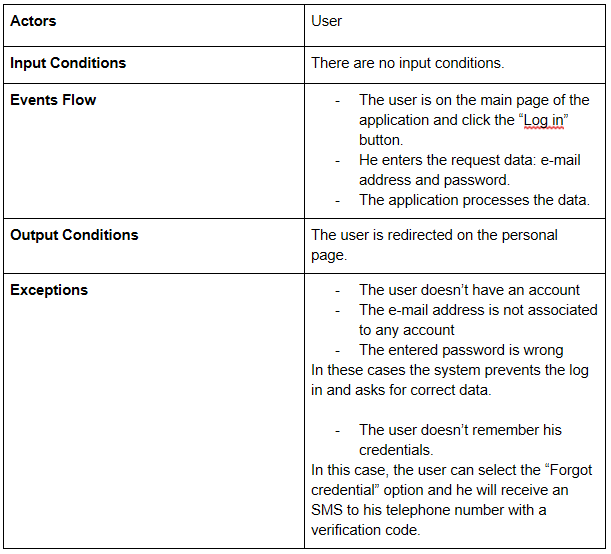
\includegraphics{Images/UseCaseTables/2_user_log.PNG}
	\caption{\label{fig:useCase2}Use case - User Login }
\end{figure}

\begin{figure}
	\centering
	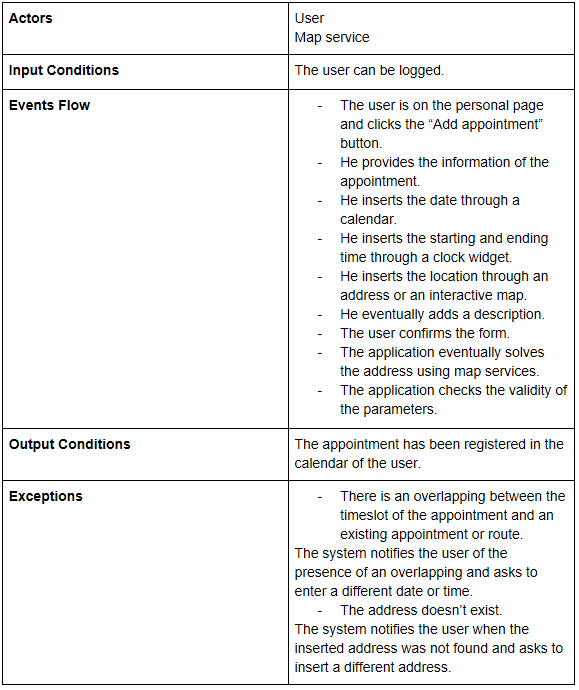
\includegraphics{Images/UseCaseTables/3_usr_add_appo.png}
	\caption{\label{fig:useCase3}Use case - User adds an Appointment }
\end{figure}

\begin{figure}
	\centering
	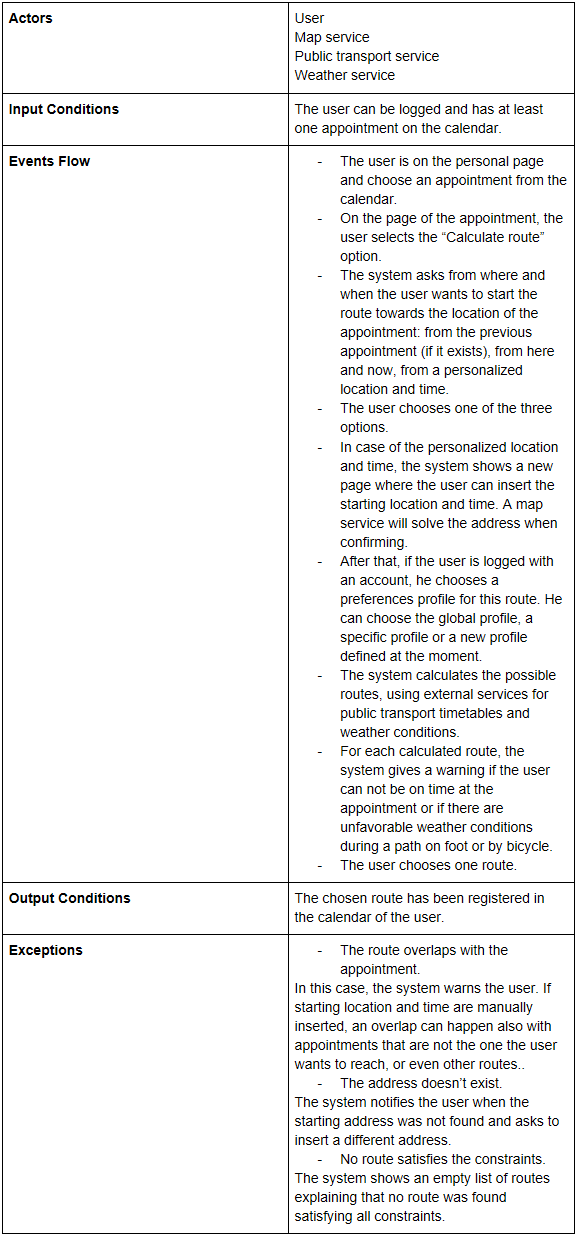
\includegraphics[totalheight=\textheight]{Images/UseCaseTables/4_The_user_add_route.png}
	\caption{\label{fig:useCase4}Use case - User adds a route to an appointment }
\end{figure}

\begin{figure}
	\centering
	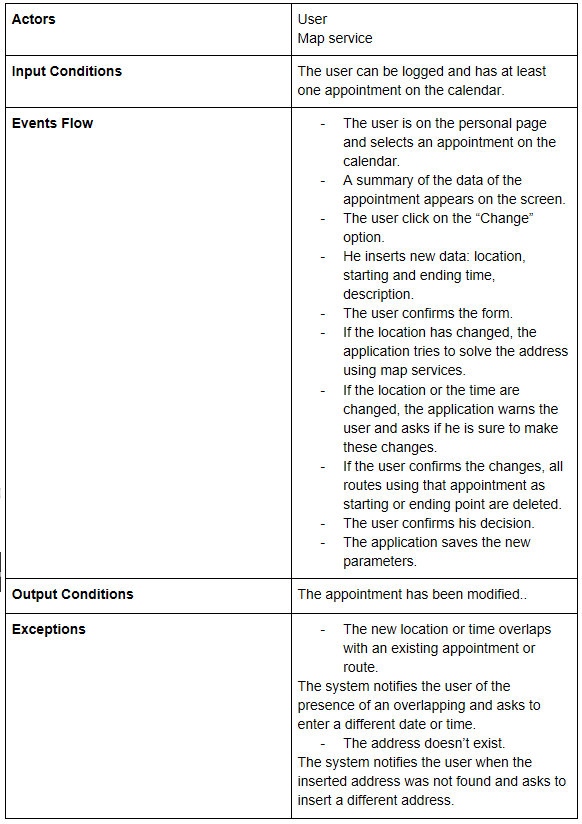
\includegraphics{Images/UseCaseTables/5_usr_changes_app.png}
	\caption{\label{fig:useCase5}Use case - User changes appointment details }
\end{figure}

\begin{figure}
	\centering
	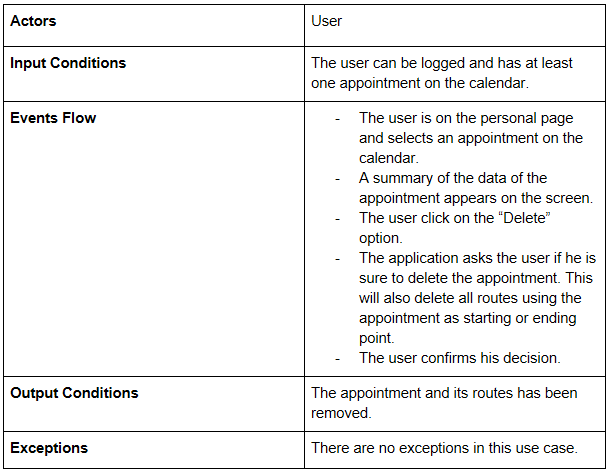
\includegraphics{Images/UseCaseTables/6_usr_del_app.PNG}
	\caption{\label{fig:useCase6}Use case - User delete appointment }
\end{figure}

\begin{figure}
	\centering
	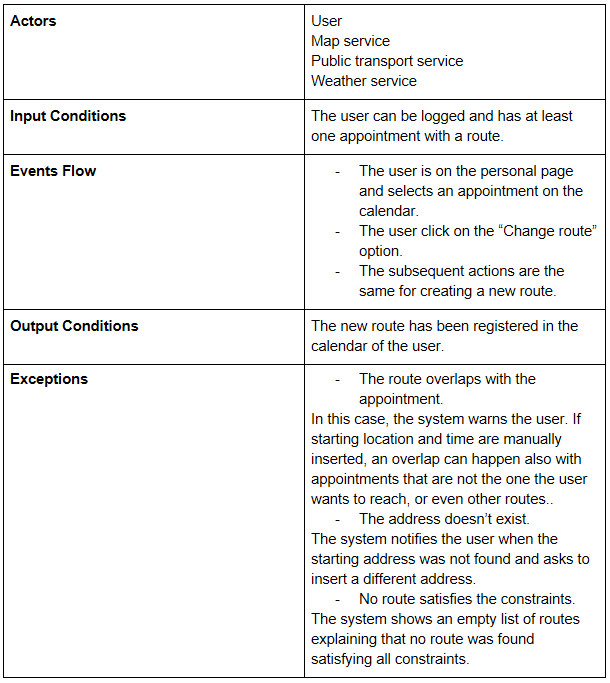
\includegraphics{Images/UseCaseTables/7_usr_mod_route.png}
	\caption{\label{fig:useCase7}Use case - User modifies a route}
\end{figure}

\begin{figure}
	\centering
	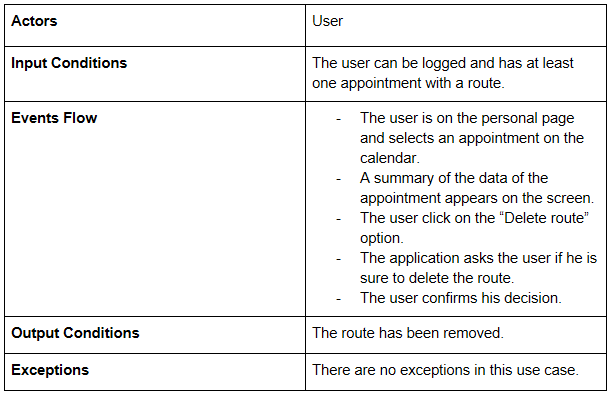
\includegraphics{Images/UseCaseTables/8_usr_del_route.PNG}
	\caption{\label{fig:useCase8}Use case - User deletes a route }
\end{figure}

\begin{figure}
	\centering
	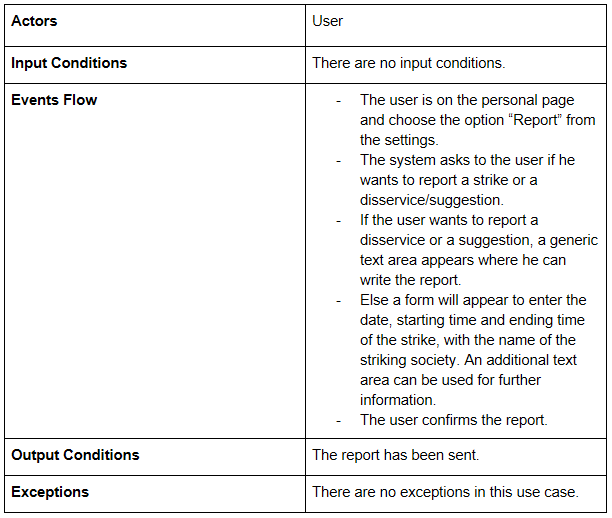
\includegraphics{Images/UseCaseTables/9_usr_report.PNG}
	\caption{\label{fig:useCase9}Use case - The user reports events and disservices  }
\end{figure}

\begin{figure}
	\centering
	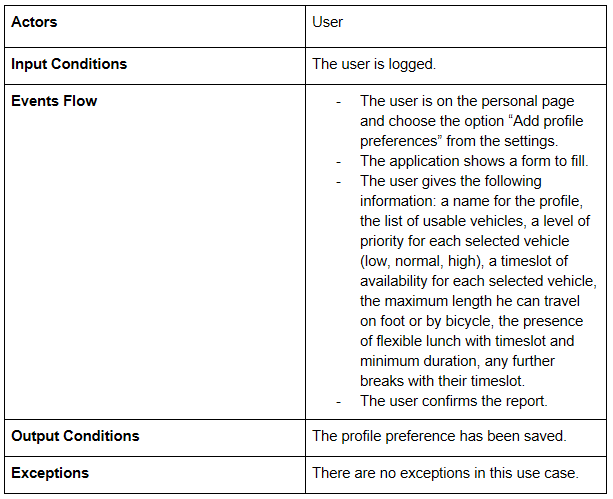
\includegraphics{Images/UseCaseTables/10_usr_add_pro_pref.PNG}
	\caption{\label{fig:useCase10}Use case - The user adds a profile preference  }
\end{figure}


\begin{sidewaysfigure}
	\centering
	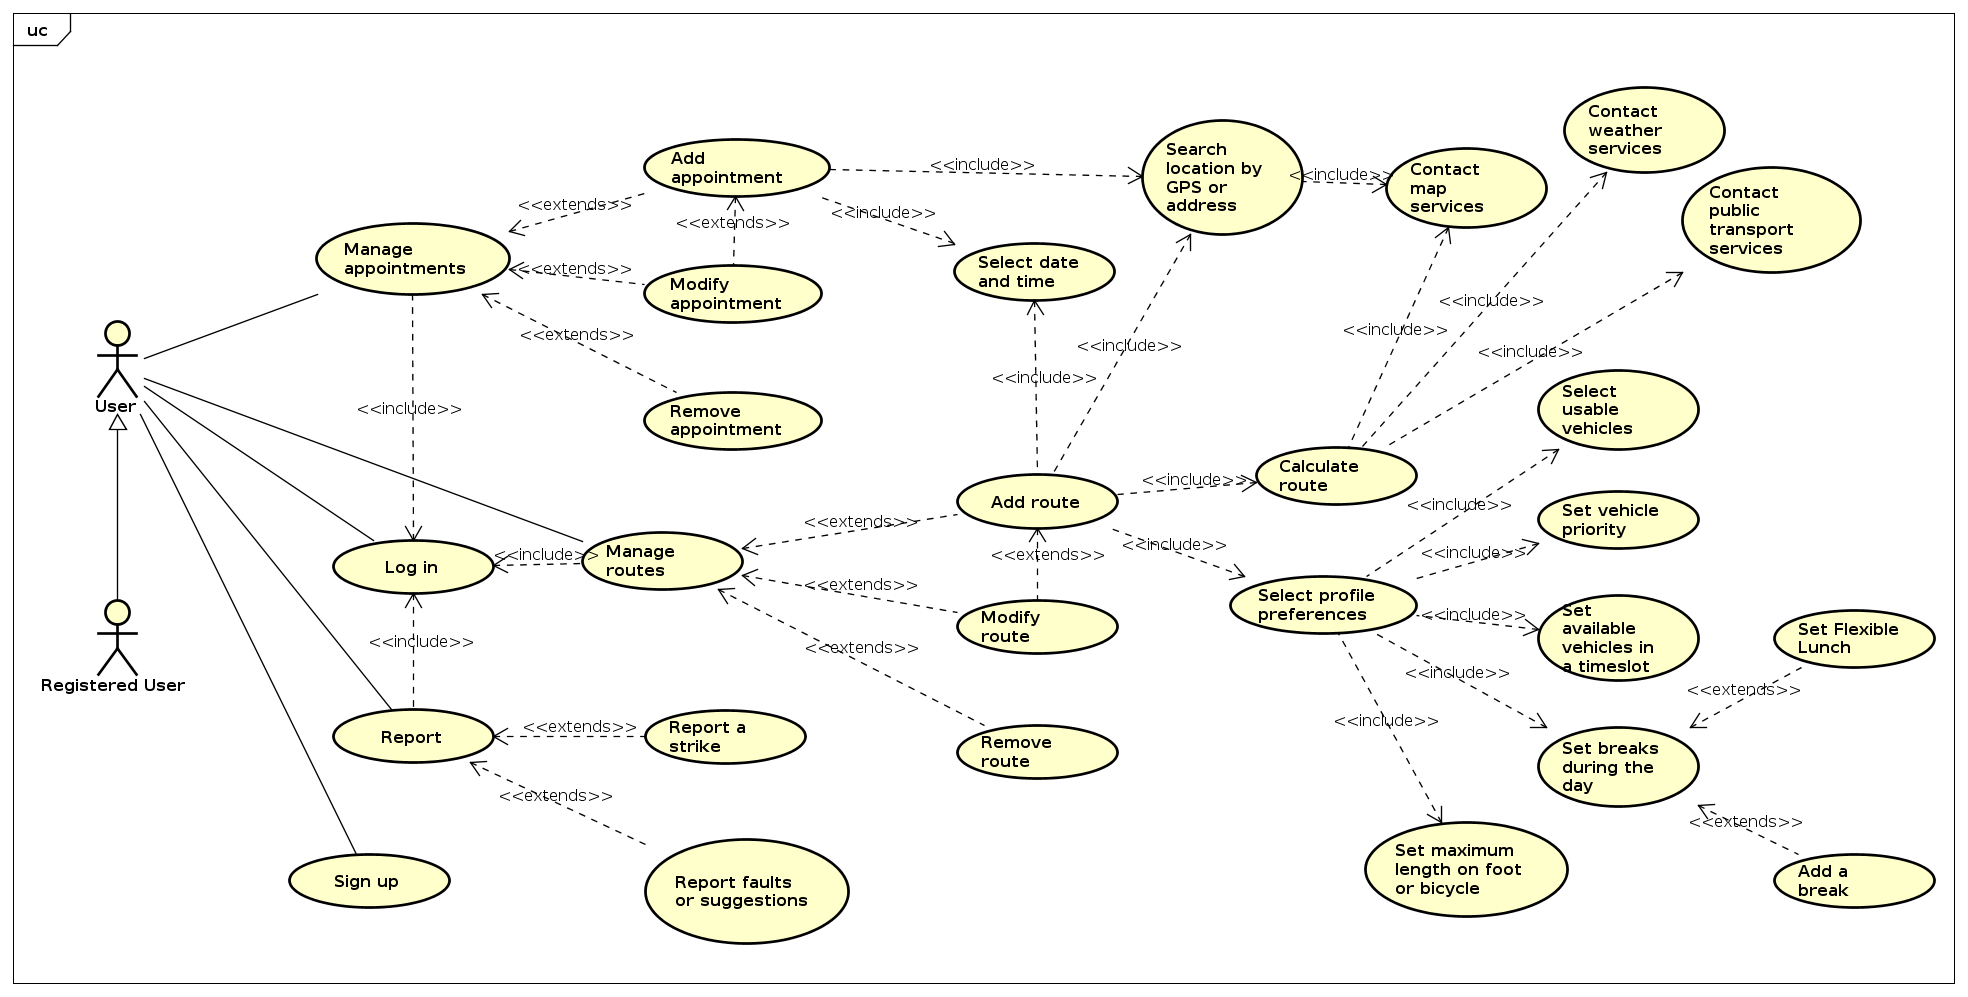
\includegraphics[width=\textwidth]{Images/UseCase_Diagram.png}
	\caption{\label{fig:useCaseDiagram}Use case diagram  }
\end{sidewaysfigure}